\appendix

\chapter{Implementation: Technology Stack and Module Inventory}
\label{app:tech_stack}

The pipeline is entirely Python-based. NER, rhetorical roles, and
summarisation run on top of \texttt{opennyai} with spaCy~3.2.4 and
CUDA-enabled PyTorch and CuPy, provisioned via a pinned micromamba
environment (\texttt{fixed\_gpu\_opennyai\_final}). Outcome labelling
uses a Mistral model invoked through a batched client script.
Multi-hearing merging is implemented in
\path{merge_cases_v3.py} under the \path{Timeline_Maker} module.
Graph construction is built on \texttt{torch\_geometric}'s
\texttt{HeteroData}, with text embeddings produced by
\path{BAAI/bge-m3} running multi-process on GPU and cached per
bucket. Training, ablation, and analysis scripts live under
\path{section_GNN}.

\chapter{Supplementary Figures from Graph Exploration}
\label{app:graph_exploration}

This appendix collects the additional structural-analysis figures
referenced from Chapter~\ref{chap:graph_exploration}, together with
the full explanatory text for each one.

\section{Shared versus Local Node Counts per Bucket}
\label{app:shared_vs_local}

Whether two cases share a node, or each hold a private copy of one,
determines whether information can flow between them through that
node. Figure~\ref{fig:shared_vs_local} breaks the per-bucket node
counts into a shared layer and a local layer. The split is sharp and
legally interpretable: party nodes (\textsc{Petitioner},
\textsc{Respondent}, most \textsc{Lawyer} nodes) are almost entirely
local, a party in one matter rarely recurs in another unrelated
case, while statutes, provisions, courts, and frequently-cited
precedents form a small but densely shared layer. This is the layer
through which all cross-case message passing must flow. Holding
judges and specific lawyers local, as the leakage-safe schema does,
does not destroy cross-case connectivity: the statute and precedent
layer remains fully intact and is the genuine information carrier.

\begin{figure}[H]
  \centering
  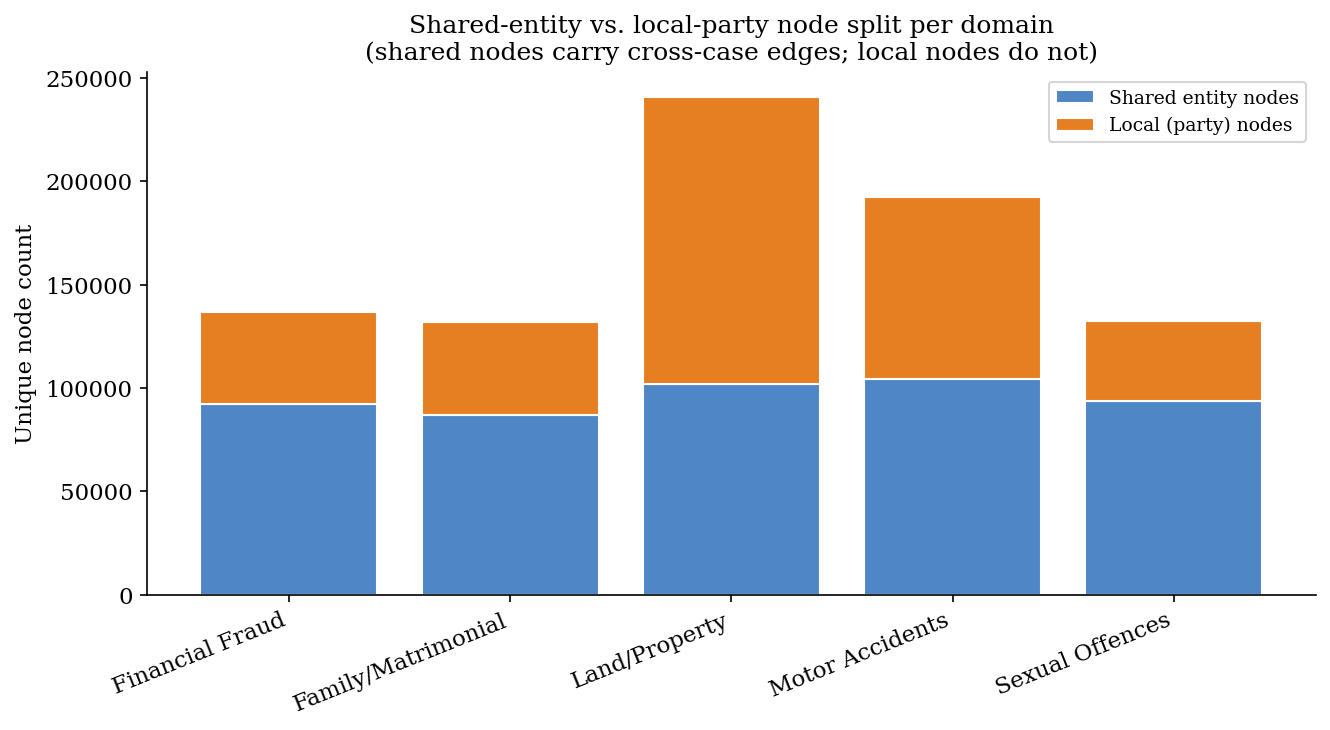
\includegraphics[width=0.92\textwidth]{figures/41_shared_vs_local_nodes_per_bucket.png}
  \caption{Shared versus local node counts per legal domain bucket.
  Party nodes are almost entirely local. Statutes, provisions, courts,
  and frequently-cited precedents form the shared layer that is the
  graph's cross-case connective tissue.}
  \label{fig:shared_vs_local}
\end{figure}

\section{Top Hub Entities: Degree and Bridging}
\label{app:top_hubs_bridging}

Figure~\ref{fig:top_hubs_bridging} plots the top hub entities by
degree alongside the number of buckets they appear in, combining both
dimensions into a single view. The two dimensions are correlated but
not identical: some high-degree nodes are concentrated within a
single domain (heavily-cited domain-specific provisions), while the
universal bridges, \textsc{IPC}, \textsc{CR.P.C.},
\textsc{Supreme Court}, top both rankings simultaneously. This
distinction matters for cross-domain transfer: only the universally
shared hubs actually mediate information flow between all five
buckets during message passing. A high-degree domain-specific hub
influences prediction accuracy within its own bucket but contributes
nothing to cross-bucket generalisation.

\begin{figure}[H]
  \centering
  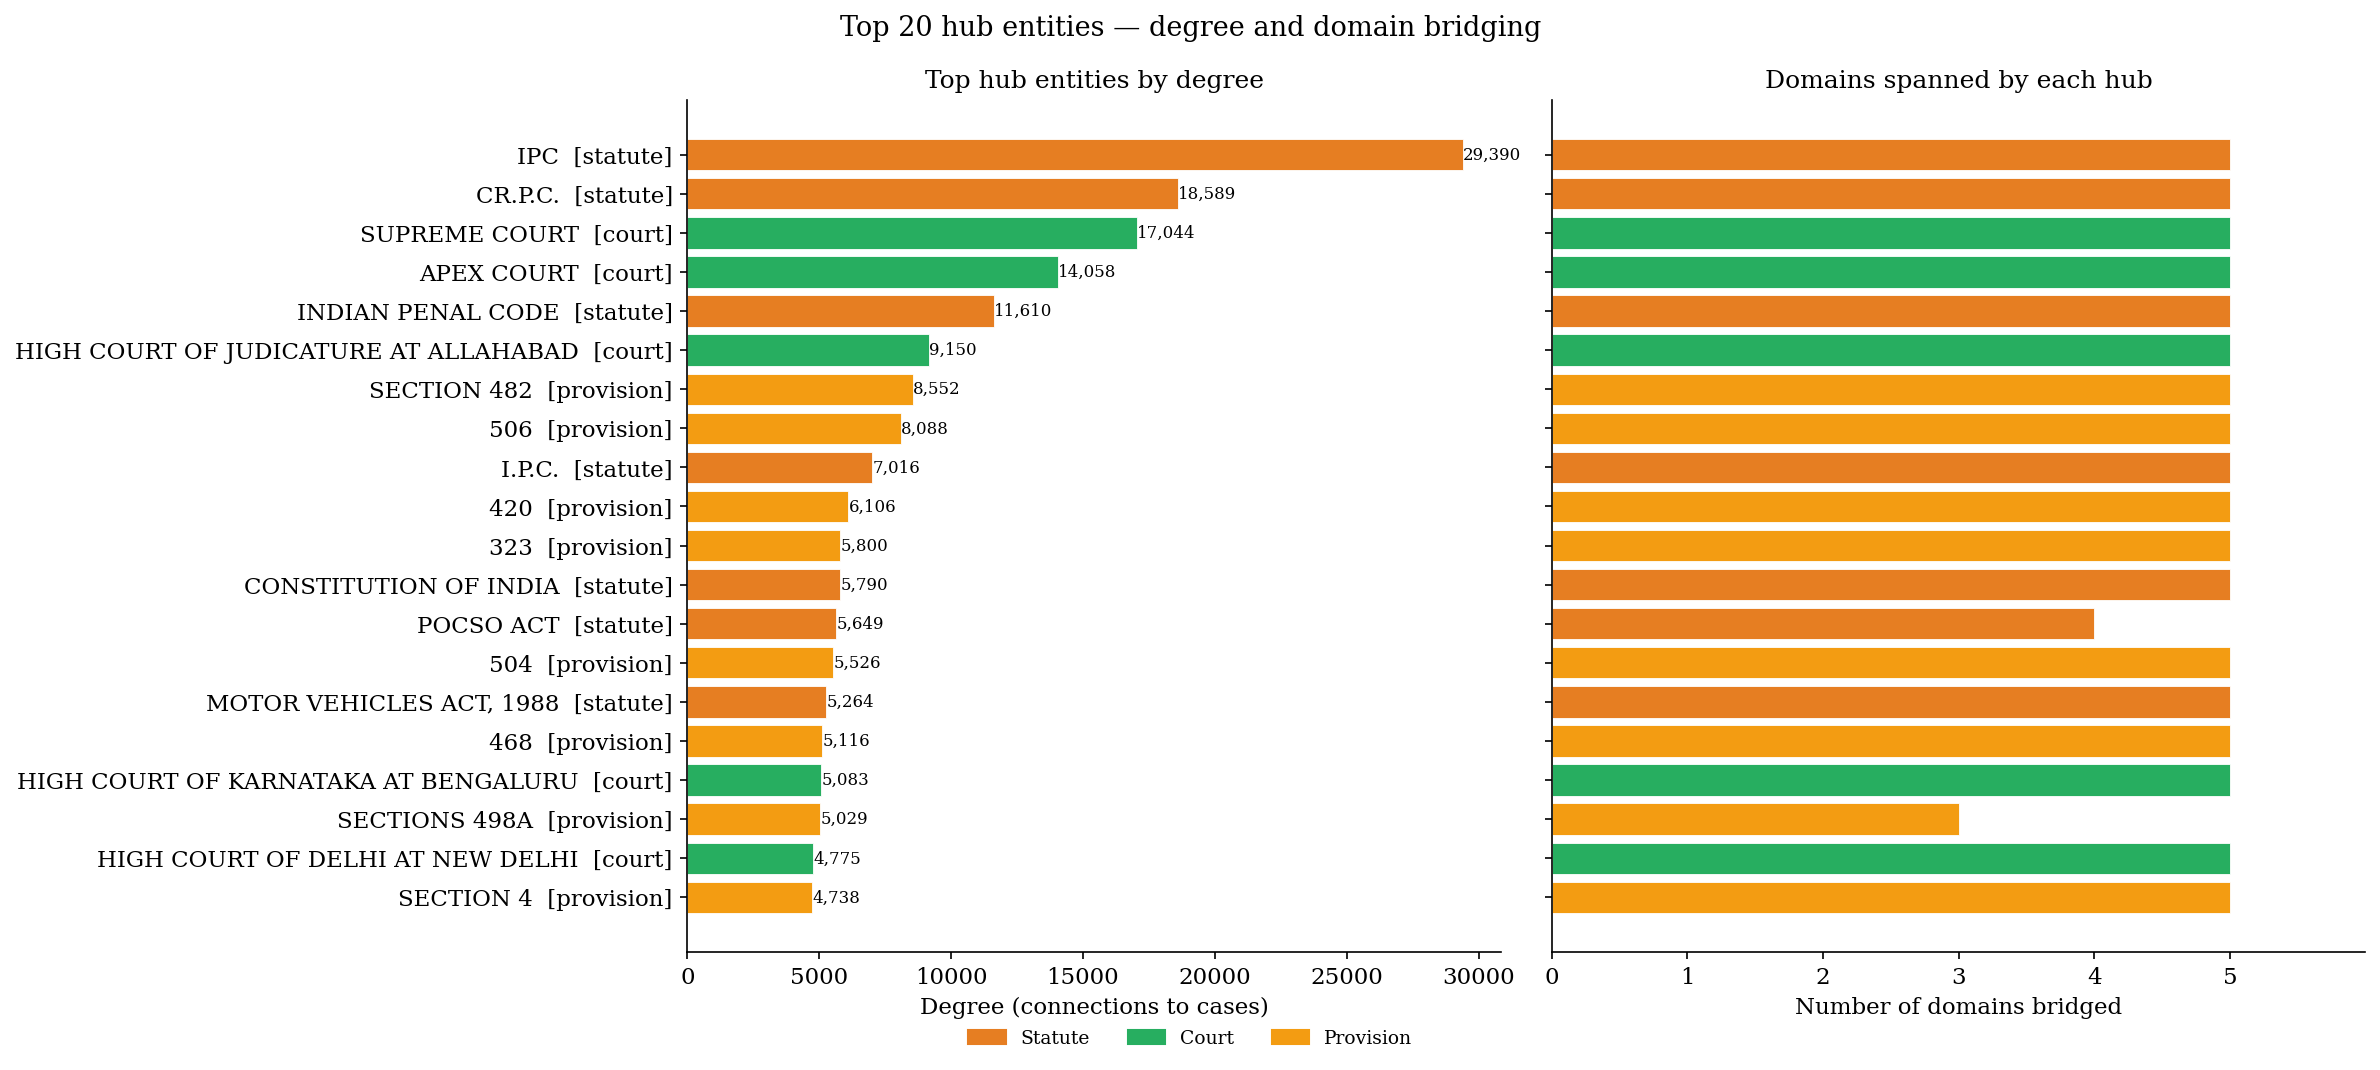
\includegraphics[width=0.92\textwidth]{figures/40_top_hubs_degree_and_bridging.png}
  \caption{Top hub entities ranked by degree, with the number of legal
  domain buckets they bridge encoded by colour or marker size. The
  universal bridges (\textsc{IPC}, \textsc{CR.P.C.}, \textsc{Supreme
  Court}) top both rankings; domain-specific high-degree hubs appear
  in fewer buckets.}
  \label{fig:top_hubs_bridging}
\end{figure}

\section{Degree Distribution (CCDF)}
\label{app:degree_ccdf}

Figure~\ref{fig:degree_ccdf} plots the complementary cumulative degree
distribution (CCDF) of the unified graph on a log-log scale. The
approximately linear decay is the signature of a heavy-tailed,
scale-free-like degree distribution: the vast majority of nodes sit
at degree one or two, while a thin upper tail extends to degrees of
tens of thousands. This two-regime structure, a small set of
super-hubs plus a long tail of single-case leaves, has a direct
modelling consequence: message passing aggregates over all
neighbours, so hub nodes receive and broadcast information from a
disproportionately large fraction of the graph. Cross-case reasoning
capacity is therefore structurally concentrated in a handful of
statute and court nodes.

\begin{figure}[H]
  \centering
  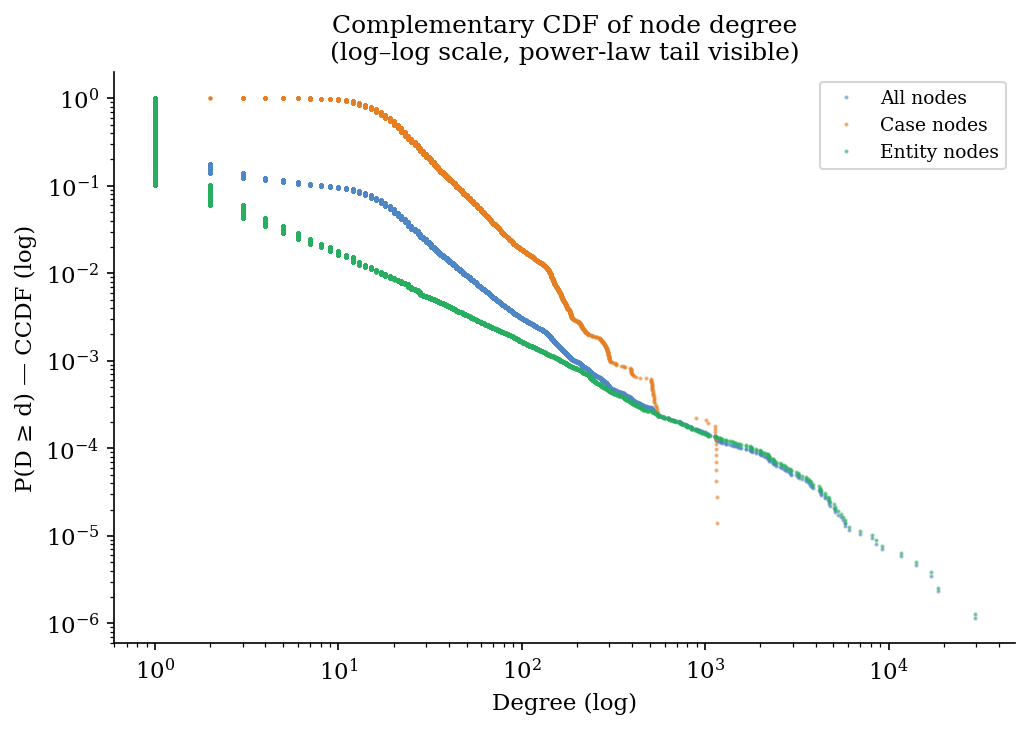
\includegraphics[width=0.92\textwidth]{figures/37_degree_ccdf_loglog.png}
  \caption{Complementary cumulative degree distribution (CCDF) of the
  unified graph on a log-log scale. The approximately linear decay
  confirms that hub dominance is a systemic structural feature rather
  than an artefact of a few outliers.}
  \label{fig:degree_ccdf}
\end{figure}

\section{Connectivity Score Distribution per Bucket}
\label{app:connectivity_violin}

A case that cites hub statutes and widely-cited precedents has many
high-degree shared neighbours and can therefore receive rich
aggregated information from a large neighbourhood during message
passing. A case that sits primarily on rare or single-occurrence
entities is structurally isolated and receives little cross-case
signal. Figure~\ref{fig:connectivity_violin} shows the per-bucket
connectivity score distribution as a violin plot, which exposes not
just the central tendency but the full distributional shape.

Land-property and financial-fraud show wider distributions with
higher medians: their cases cite diverse authorities and are
therefore well-connected to the hub layer. Motor-accidents shows a
narrow distribution concentrated at low values, reflecting the
domain's repeated citation of the same small provision set
(\textsc{Motor Vehicles Act}, Section~166). The within-bucket
variance is itself informative: even within a single domain, cases
span a substantial connectivity range, meaning that prediction
difficulty is heterogeneous at the case level and cannot be
attributed to domain alone. The ablation pattern in
Chapter~\ref{chap:results} is consistent with this expectation: cases
in the low-connectivity tail of any bucket show systematically higher
error rates.

\begin{figure}[H]
  \centering
  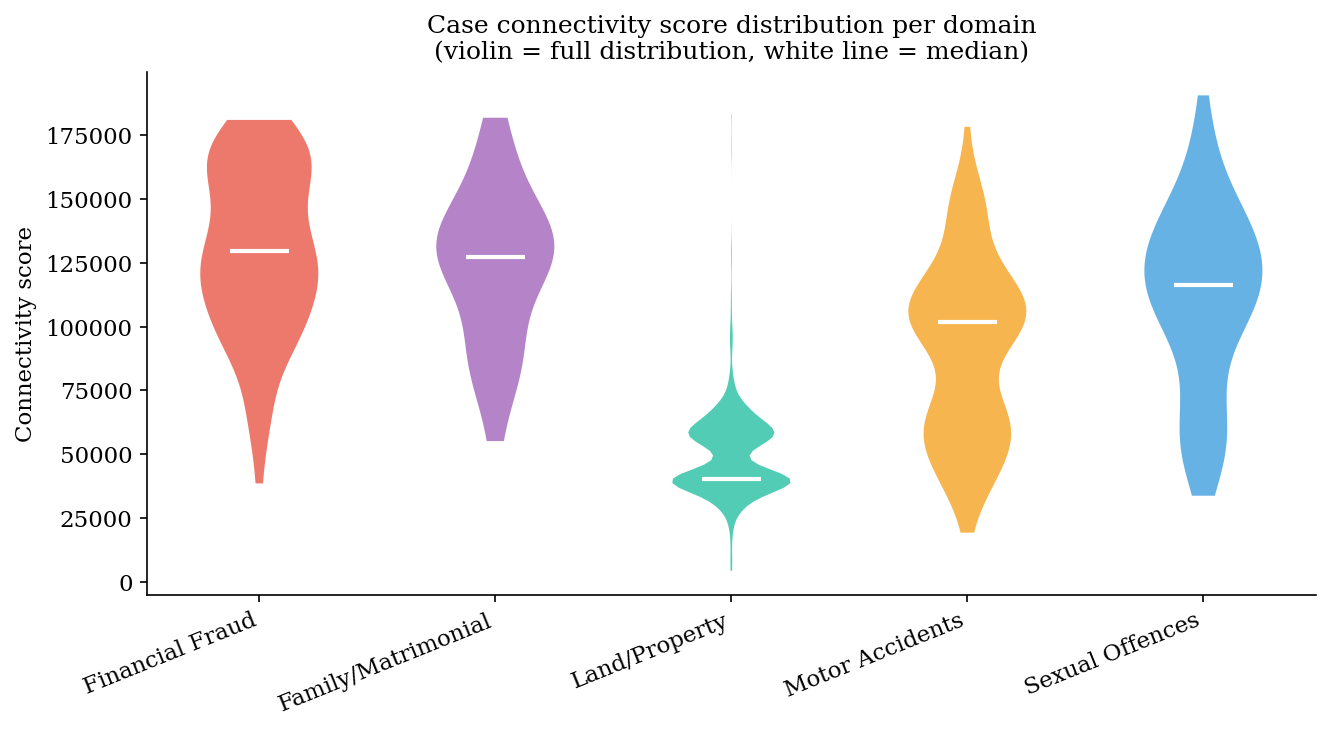
\includegraphics[width=0.9\textwidth]{figures/39_connectivity_violin.png}
  \caption{Per-bucket connectivity score distribution as violin plots.
  Land-property and financial-fraud are wider and higher-median;
  motor-accidents is narrowly concentrated at low values.}
  \label{fig:connectivity_violin}
\end{figure}

\section{Sentence-Count Distribution per Bucket}
\label{app:sentence_count_dist}

Case length varies substantially across buckets, and that variance
directly determines how text features are constructed for the GNN.
Long documents require chunked embedding strategies; short documents
can be embedded whole. Motor-accidents judgments are typically short
and tribunal-style, concentrated well below 100 sentences.
Land-property matters are long and document-heavy (deeds, surveys,
possession history), with a pronounced right tail extending into
several hundred sentences per case. Financial-fraud and
family-matrimonial sit between these extremes. These distributions
are the primary driver of the hierarchical-chunking configuration in
Section~\ref{sec:text_features}: long-tail \textsc{Facts} and
\textsc{Arguments} sections in land-property and financial-fraud
buckets exceed the \texttt{bge-m3} context window and are mean-pooled
across overlapping chunks, with the chunk boundary set per-bucket
based on the 90th-percentile sentence count.

\begin{figure}[H]
  \centering
  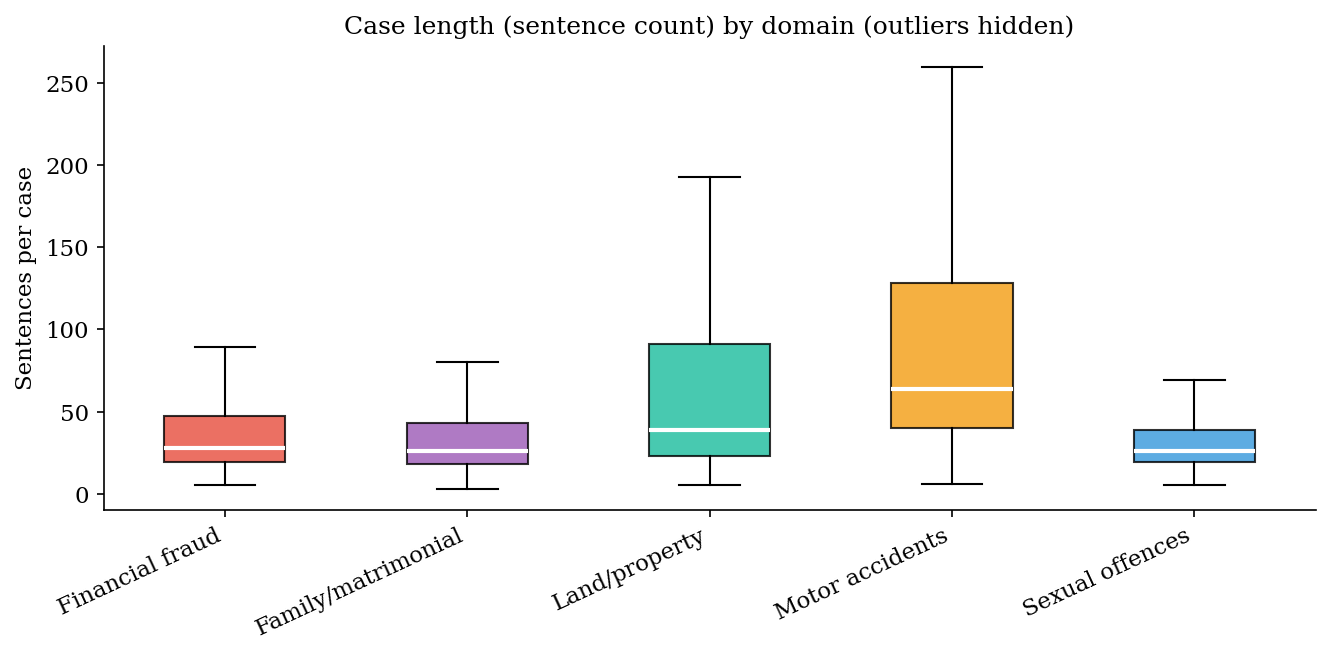
\includegraphics[width=0.92\textwidth]{figures/06_sentence_count_distribution_full.png}
  \caption{Sentence-count distribution per legal domain bucket across
  the full corpus. Land-property and financial-fraud have the heaviest
  right tails; motor-accidents is concentrated at low sentence
  counts.}
  \label{fig:sentence_count_dist}
\end{figure}

\section{Entity Richness and Mean Case Degree per Bucket}
\label{app:richness_and_degree}

Entity richness, the number of unique canonicalised entities per
case, is a per-domain structural property that predicts both graph
density and expected modelling difficulty. A domain where every case
cites a wide variety of distinct statutes, provisions, and precedents
will produce a denser, more richly interconnected subgraph; a domain
where cases repeatedly cite the same small set of authorities will
produce a sparser subgraph with lower information diversity per case.
Figure~\ref{fig:richness_and_degree} confirms the expected ordering.
Land-property and financial-fraud score highest on both axes: their
cases cite many distinct statutes, provisions, and precedents and are
therefore well-connected to the graph's shared-entity layer.
Motor-accidents scores lowest on both: it repeatedly cites the same
narrow provision set (\textsc{Motor Vehicles Act~1988}, Section~166)
and produces cases with comparatively few graph edges. The
correlation between richness and degree is expected, a case that
cites many distinct authorities will naturally have more edges,
but the per-domain consistency confirms that this is a domain-level
structural phenomenon rather than variance driven by outlier cases.
Domains with high richness and degree will benefit more from
multi-hop message passing than sparse domains; the ablation in
Chapter~\ref{chap:results} tests this prediction directly.

\begin{figure}[H]
  \centering
  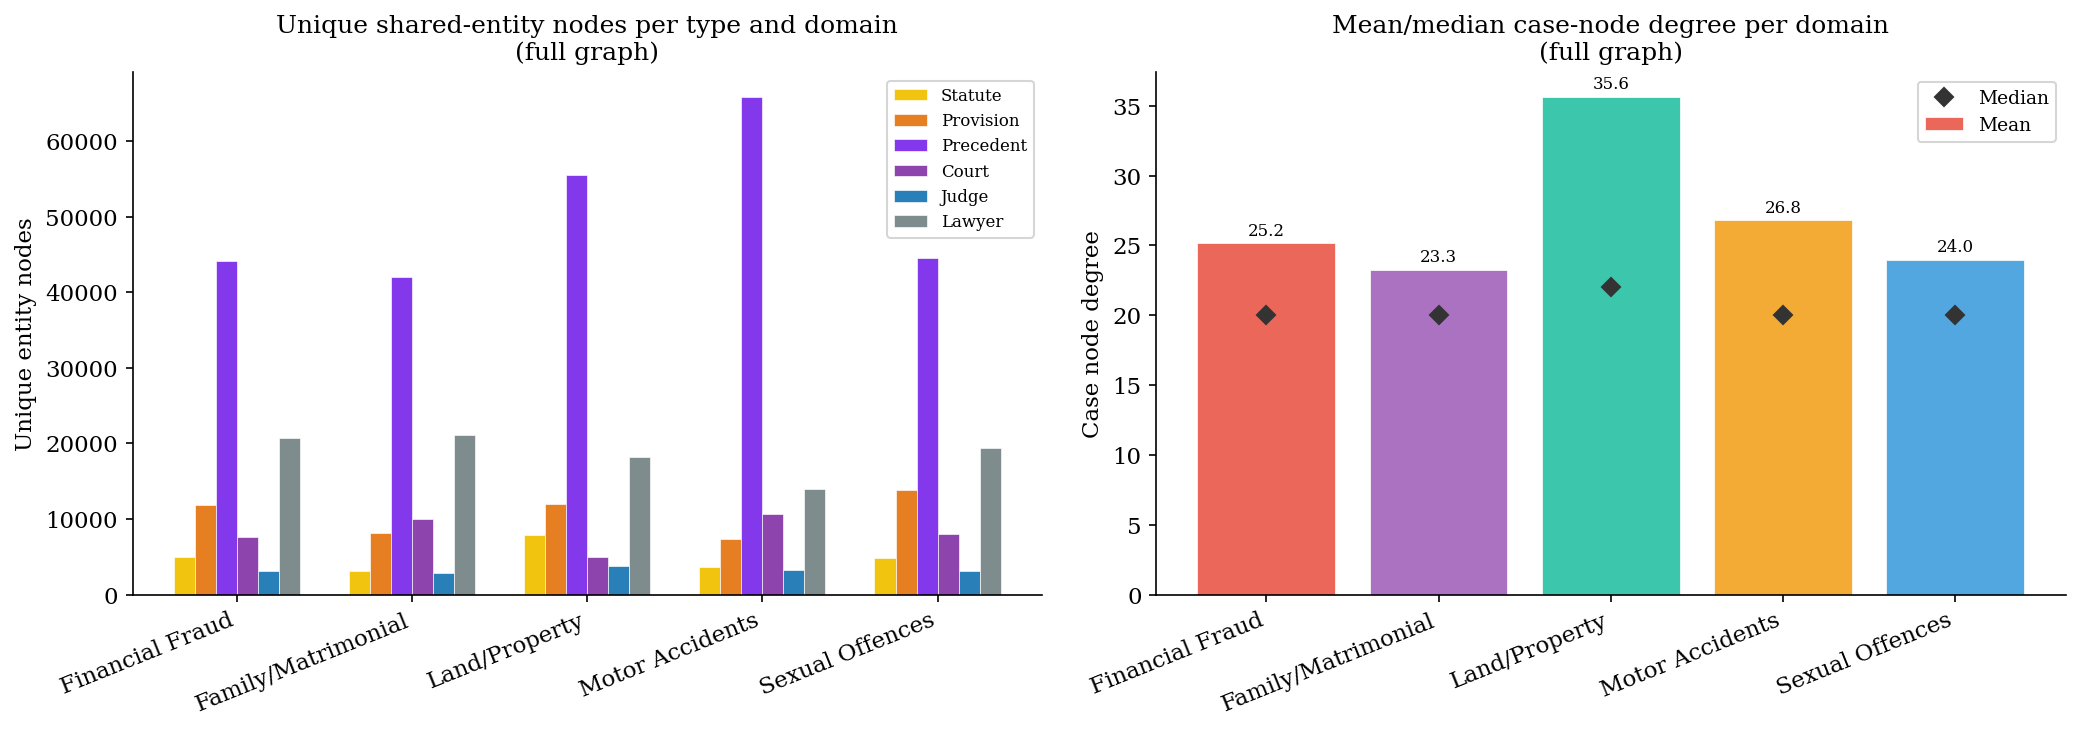
\includegraphics[width=0.92\textwidth]{figures/38_per_bucket_richness_and_degree.png}
  \caption{Entity richness (unique canonicalised entities per case)
  and mean case degree per legal domain bucket. Land-property and
  financial-fraud are entity-rich and highly connected;
  motor-accidents is entity-poor and low-degree.}
  \label{fig:richness_and_degree}
\end{figure}

\section{Within-Bucket Entity Co-occurrence Networks}
\label{app:within_bucket_network_fingerprints}

The ranked PageRank lists in Section~\ref{sec:perdomain} tell us
which entities are important within each bucket; they do not tell us
how those entities are organised relative to each other.
Figure~\ref{fig:within_bucket_network_fingerprints} makes that
geometry visible by showing the entity co-occurrence network within
each bucket restricted to its top-25 PageRank entities.

The networks reveal that the domains differ not only in their top
entities but in their network geometry, and the differences are
legally interpretable. Family~\&~matrimonial and sexual offences both
remain visibly \textsc{IPC}/\textsc{CrPC}-centred, yet they bifurcate
into distinct provision clusters almost immediately below the top
hub: Section~498A, 482, and dowry-related citations form the inner
ring in family-matrimonial, while \textsc{POCSO}, Section~376, and
Section~363 dominate in sexual offences. The two domains share the
same criminal-procedure spine but are routed through different
specialised provisions, exactly the relationship predicted by the
entity-sharing matrix
(Figure~\ref{fig:cross_bucket_sharing_matrix}).

Land-property is geometrically distinct: its network is spatially
spread with several semi-central statutory and constitutional nodes
rather than one overwhelmingly dominant criminal-procedure core. The
\textsc{Land Acquisition Act~1894} and the \textsc{Constitution of
India} sit as co-equal secondary hubs alongside \textsc{Supreme
Court}, forming a multi-centred structure consistent with the
domain's higher entity richness.

Motor-accidents, by contrast, exhibits the tightest and most
repetitive local backbone of all four domains, with \textsc{Motor
Vehicles Act~1988} and Section~166 forming an extremely compact
star. The near-absence of peripheral nodes confirms that most
motor-accidents cases enter the graph through the same narrow set of
recurring authorities, leaving little structural diversity for
multi-hop message passing to exploit.

\begin{figure}[H]
  \centering
  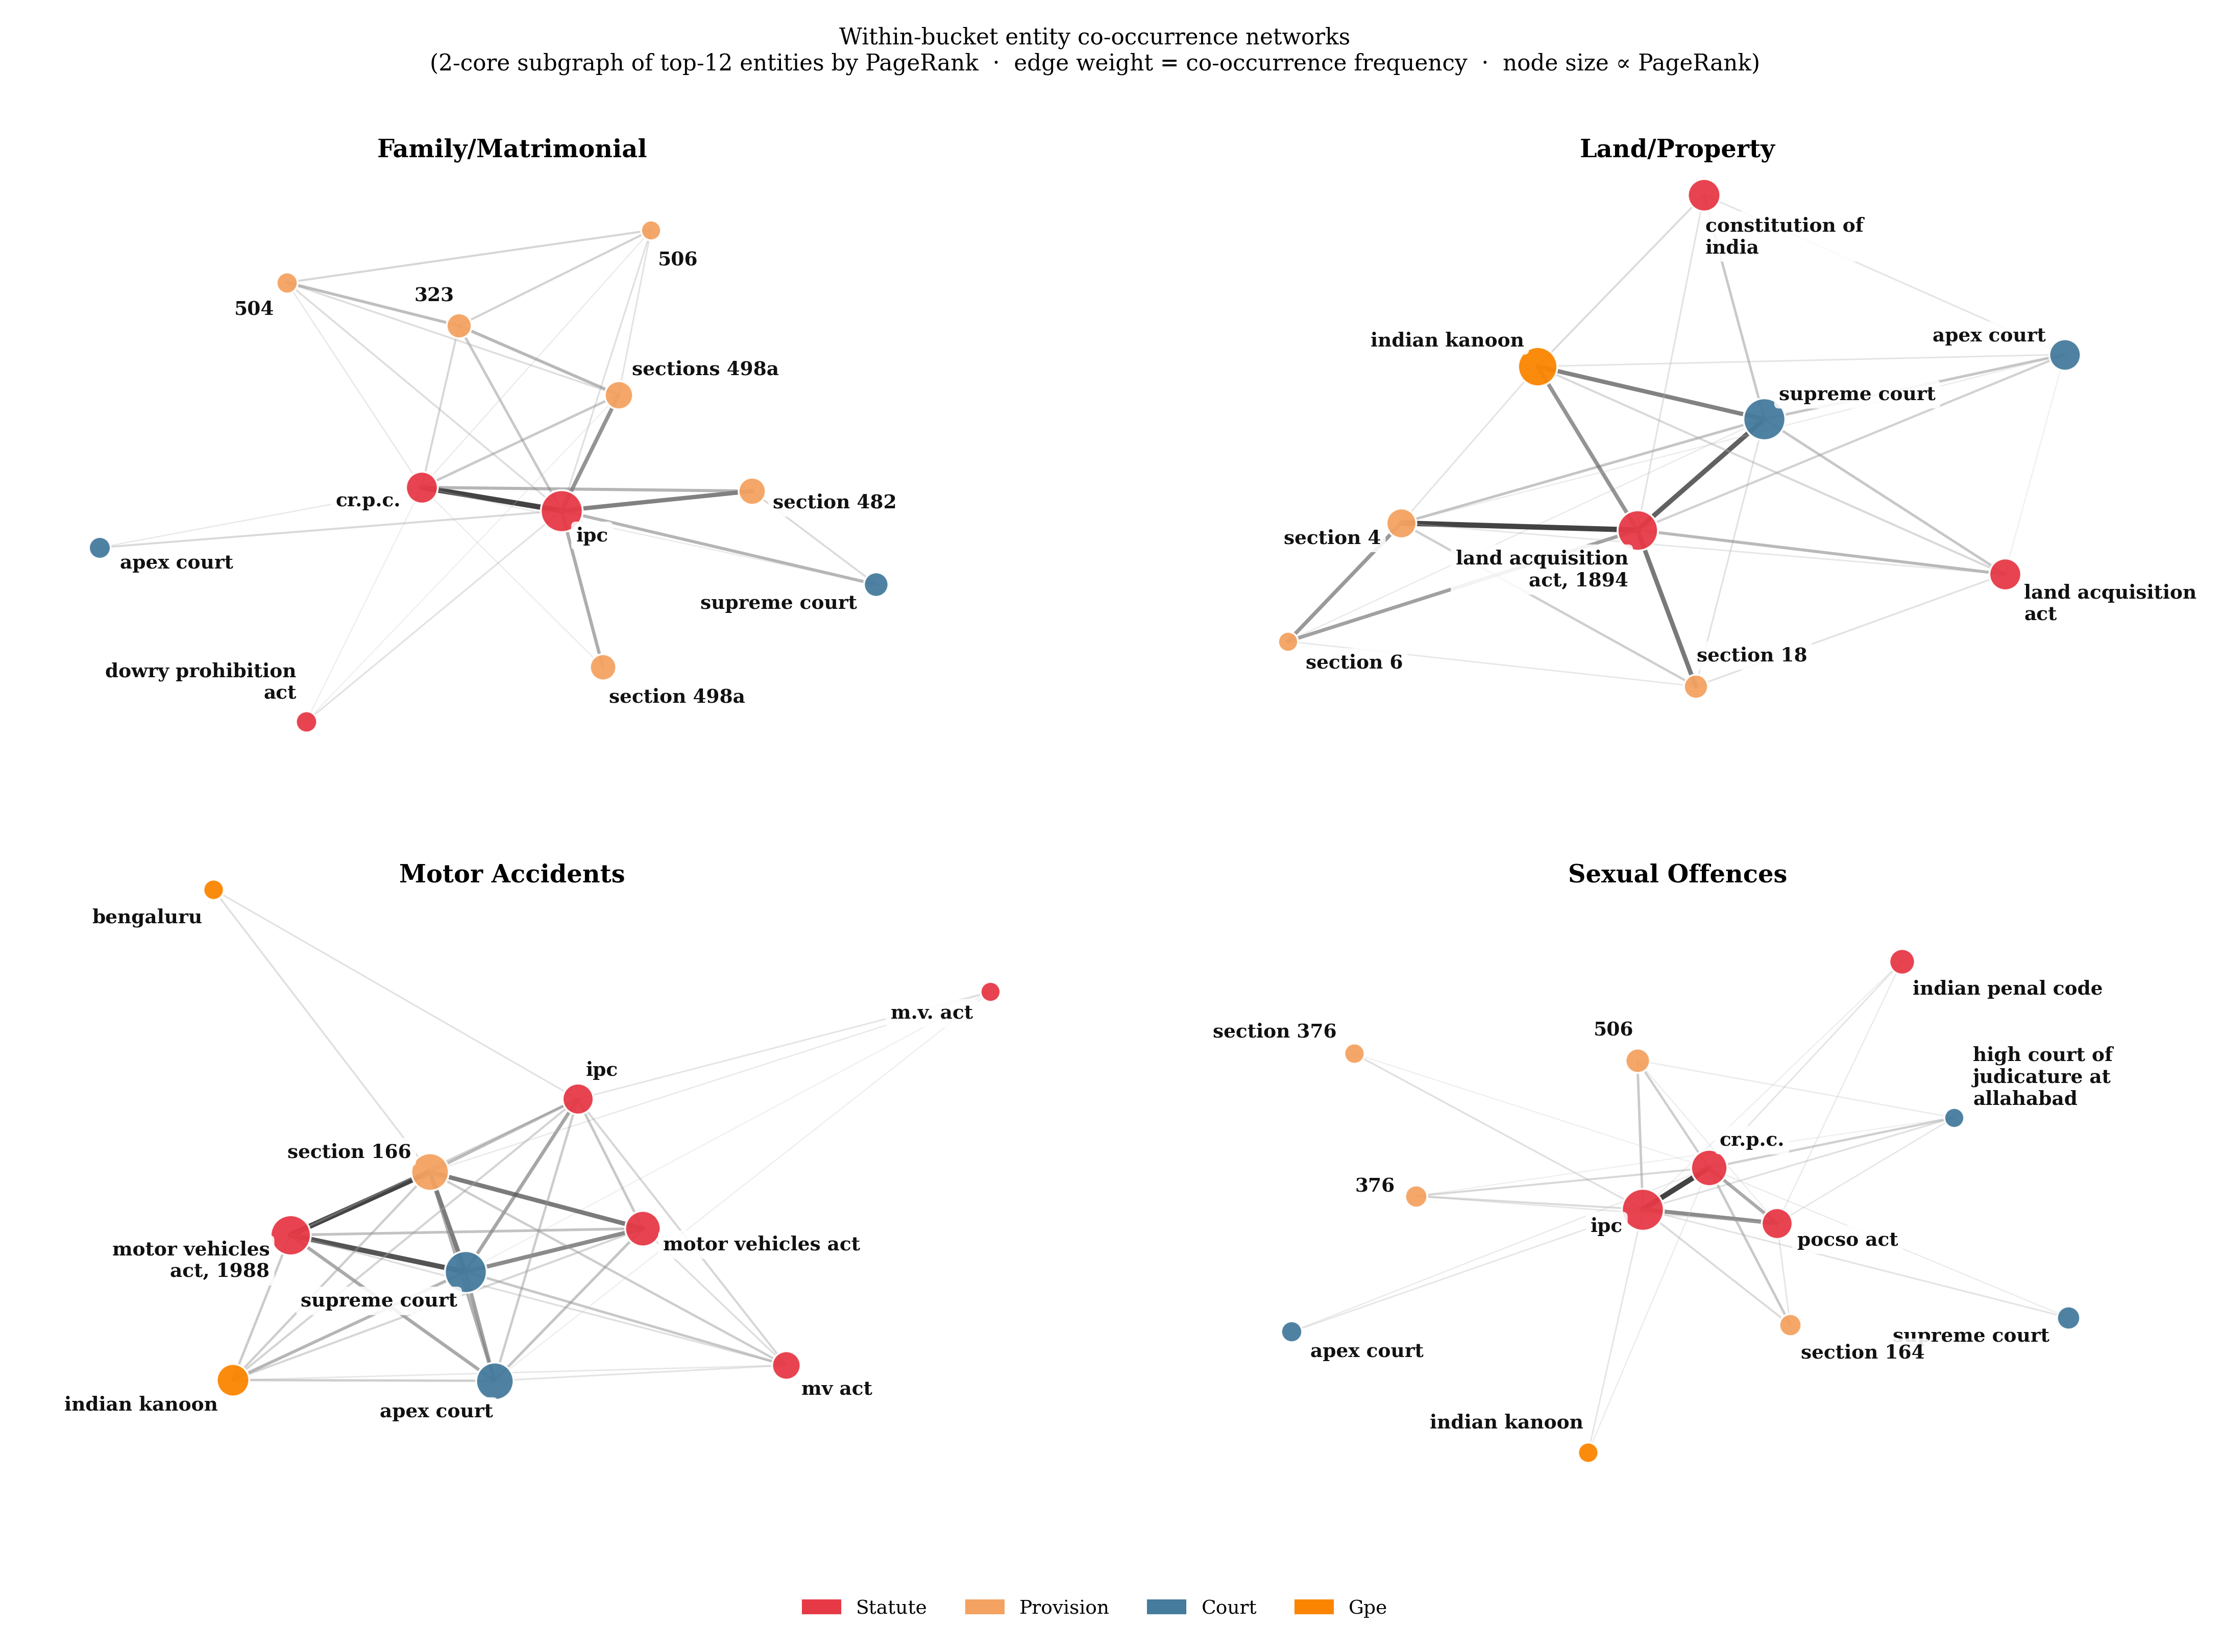
\includegraphics[width=\textwidth]{figures/36_within_bucket_network_fingerprints.png}
  \caption{Within-bucket entity co-occurrence networks for four legal
  domains, each restricted to the top-25 PageRank entities in that
  bucket. Node size is proportional to PageRank score.}
  \label{fig:within_bucket_network_fingerprints}
\end{figure}

\section{Cross-Domain Entity Fingerprint}
\label{app:cross_domain_network_fingerprint}

Figure~\ref{fig:cross_domain_network_fingerprint} collapses the five
within-bucket networks into a single cross-domain graph. Each domain
is represented as a large hub node placed at a vertex of a pentagon;
the top-10 PageRank entities from each domain appear as satellite
nodes connected to whichever hubs they belong to. Entities that
appear in the top-10 of two or more domains are drawn with a bold
outline and linked by crimson cross-domain edges, making the
inter-domain bridges immediately legible.

The cross-domain view reveals a clear three-tier bridge structure.
At the widest tier, \textsc{Supreme Court} and \textsc{Apex Court}
appear in the top-10 of all five domains, universal procedural
anchors that carry interpretive weight regardless of substantive
legal area. At the intermediate tier, \textsc{IPC}, \textsc{CrPC},
and \textsc{Section~482} bridge the three criminal-procedure domains
(Family/Matrimonial, Financial Fraud, and Sexual Offences) but are
absent from the top tier of Land/Property and Motor Accidents,
confirming that the criminal-procedure spine is real but
domain-bounded. At the narrowest tier, domain-exclusive entities
(\textsc{Land Acquisition Act~1894} for land-property, \textsc{Motor
Vehicles Act~1988} and \textsc{Section~166} for motor-accidents,
\textsc{POCSO} for sexual offences) remain firmly segregated. This
stratified bridge structure is precisely what a well-designed
heterogeneous graph should exhibit: enough shared structure for
cross-domain representation learning, but enough domain exclusivity
to recover meaningful per-domain fingerprints rather than collapsing
all five into a single undifferentiated embedding.

\begin{figure}[H]
  \centering
  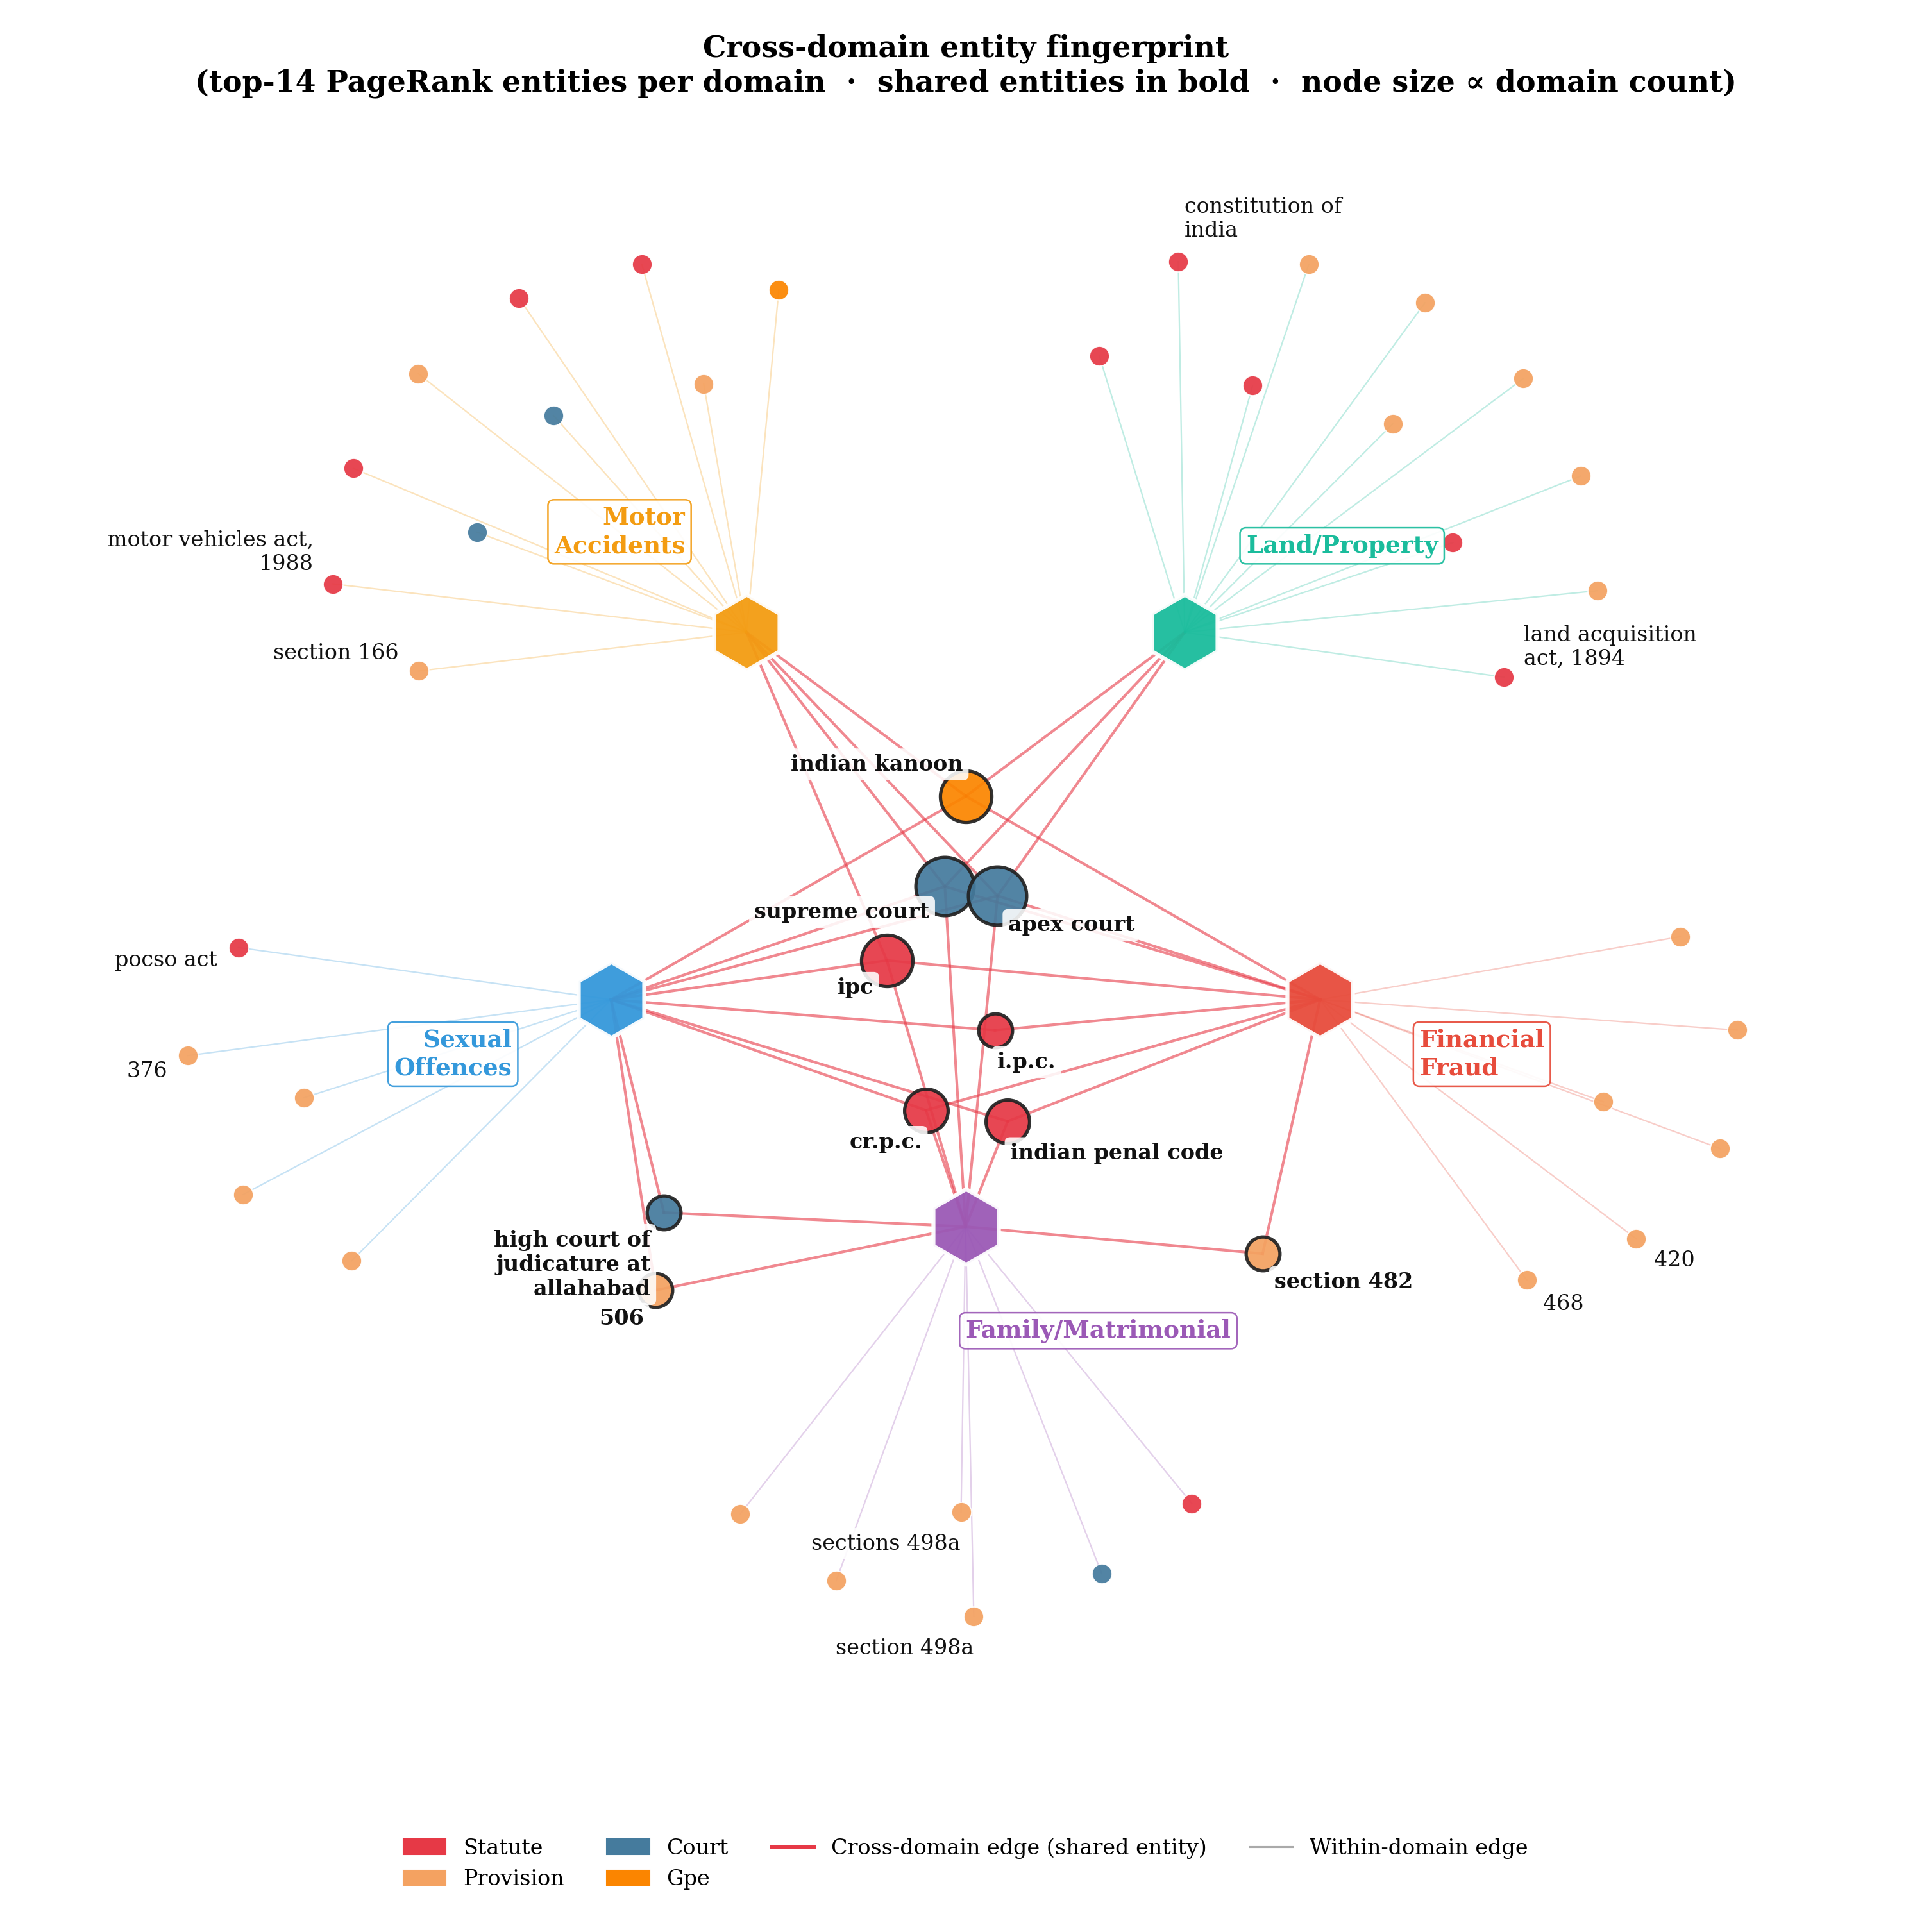
\includegraphics[width=\textwidth]{figures/44_cross_domain_network_fingerprint.png}
  \caption{Cross-domain entity fingerprint. Node colour encodes
  entity type; node size encodes the number of domains the entity
  appears in. Crimson edges connect entities that bridge two or more
  domains; domain-coloured edges connect exclusive entities to their
  single hub.}
  \label{fig:cross_domain_network_fingerprint}
\end{figure}

\chapter{Supplementary Figures from Interpretability Analysis}
\label{app:explainability}

This appendix collects the interpretability figures referenced from
Chapter~\ref{chap:explainability}, with full explanatory text for
each.

\section{Node-Type Importance via Input Zeroing}
\label{app:node_importance}

For each node type in turn, all features of that type are replaced
with zeros and the frozen HGT is re-evaluated; the drop in test
accuracy is the node type's importance. Because the graph topology
is preserved, this isolates the \emph{featural} contribution of each
type. On the cross-bucket baseline (fold~0, baseline accuracy
$0.8134$) the ranking is:
\textsc{Case} ($-0.0430$) $\gg$
\textsc{Arguments} ($-0.0173$) $>$
\textsc{Petitioner} ($-0.0130$) $>$
\textsc{Other\_Lawyer\_Arguments} ($-0.0093$) $>$
\textsc{Judge} ($-0.0084$) $>$
\textsc{Respondent\_Arguments} ($-0.0058$) $>$ remaining types
$\leq\!0.0032$; statute zeroing is within noise of baseline.

Two readings are worth making explicit. First, the model remains
\emph{anchored in the case node itself}: its own text features are
the dominant source of information, consistent with reading the
classifier out from the \textsc{Case} representation. Second, the
remaining signal is distributed across the argument stream and the
immediate participants (\textsc{Petitioner},
\textsc{Other\_Lawyer\_Arguments}, \textsc{Judge}) rather than
concentrated on any single authority type, individual
\textsc{Statute} and \textsc{Provision} nodes have near-zero per-type
importance, so the cross-case signal they carry flows through the
arguments rather than directly through statutory features.

\begin{figure}[H]
  \centering
  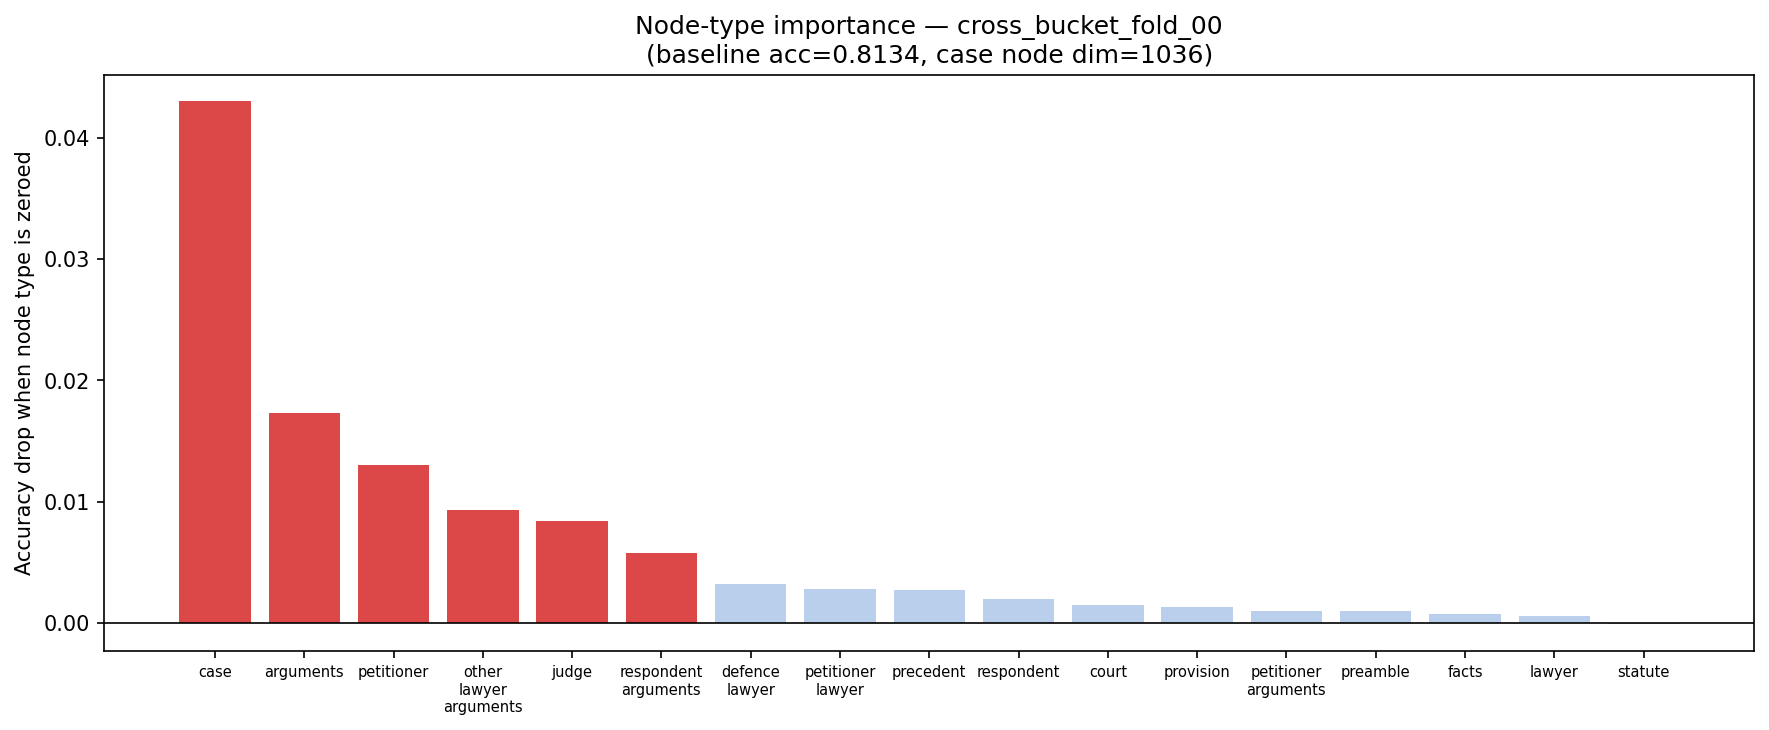
\includegraphics[width=0.78\linewidth]{figures/explainability/node_importance.png}
  \caption{Node-type importance via input zeroing on the cross-bucket
  baseline, fold~0. Each bar is the accuracy drop when the listed
  node type's features are zeroed before forward pass, holding the
  graph and the remaining features constant.}
  \label{fig:node_importance}
\end{figure}

\section{Per-Relation Attention and Gradient Saliency}
\label{app:attention_saliency}

Two patterns emerge consistently from the attention and saliency
probes. First, the \path{rev_has_*} edges, those carrying
information \emph{from} text and entity nodes \emph{back to} the case
node, hold systematically higher attention mass than their forward
counterparts. This is consistent with the architecture: the
classifier reads only the \textsc{Case} node's final representation,
so a neighbour's value is measured by how strongly the reverse edge
delivers it. Second, gradient saliency ranks node types as
\textsc{Case} $\gg$ \textsc{Arguments} $>$
\textsc{Other\_Lawyer\_Arguments} $>$ \textsc{Respondent\_Arguments}
$>$ \textsc{Facts} $>$ \textsc{Judge} $>$ \dots, mirroring the
zeroing ranking and confirming that the argument stream is the
operational hinge of the model.

\begin{figure}[H]
  \centering
  \begin{minipage}{0.49\textwidth}
    {\footnotesize (a) Per-relation attention heatmap\par}
    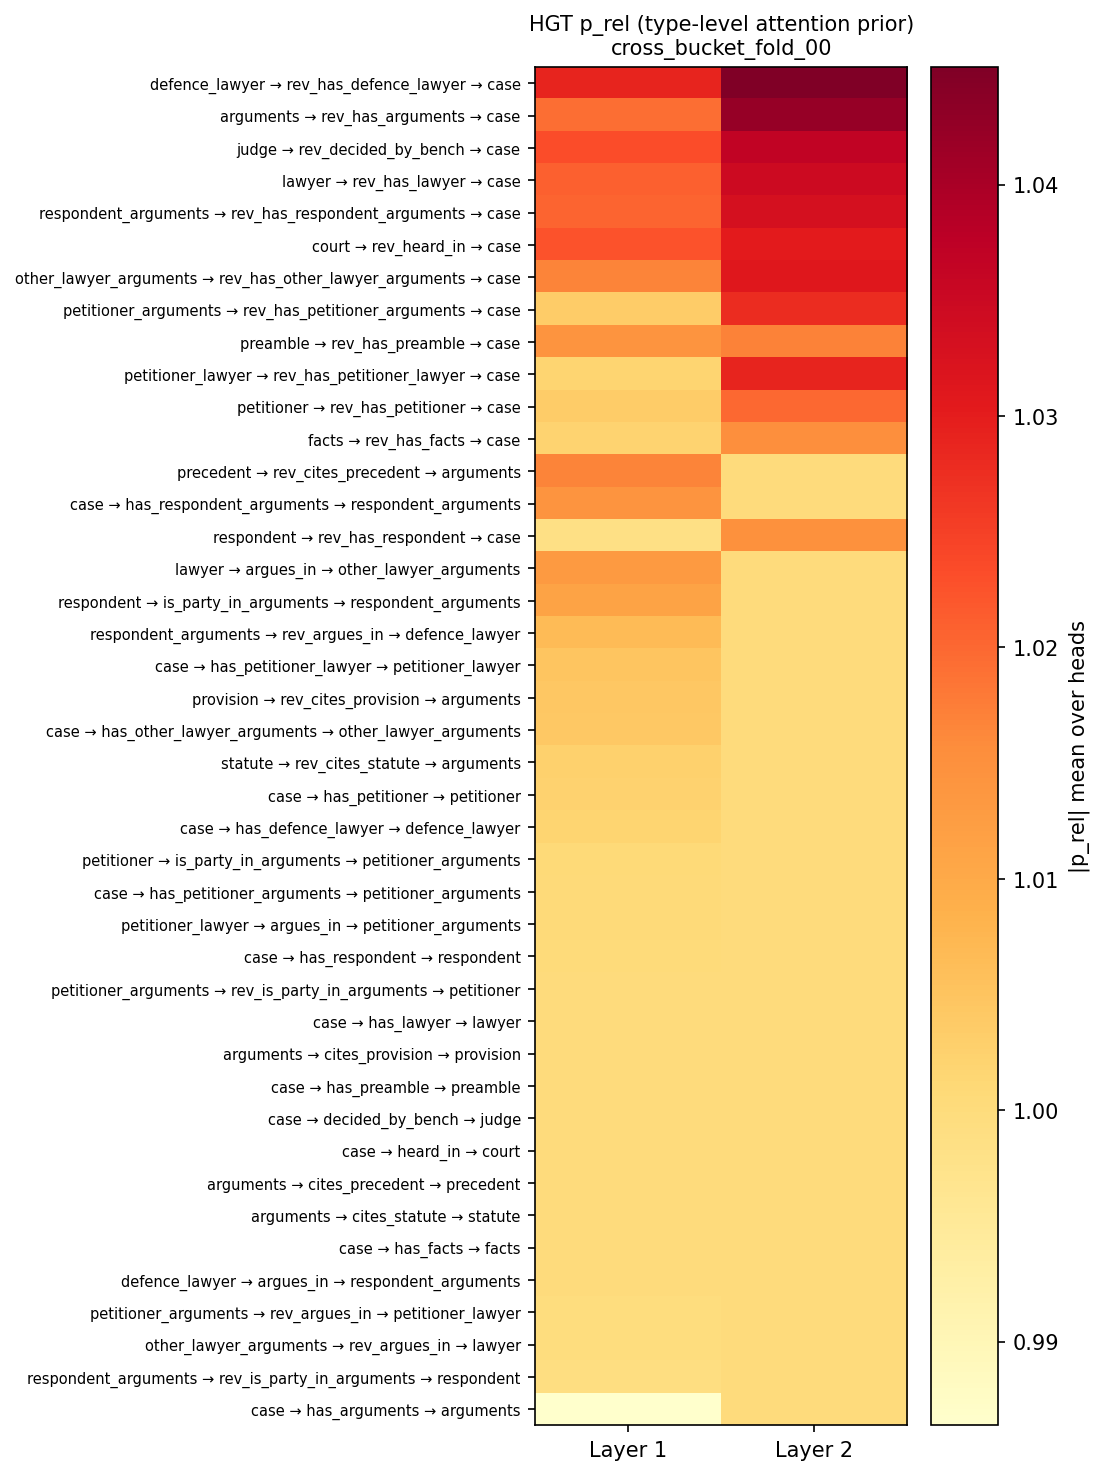
\includegraphics[width=\linewidth]{figures/explainability/prel_heatmap.png}
  \end{minipage}\hfill
  \begin{minipage}{0.49\textwidth}
    {\footnotesize (b) Gradient saliency by node type\par}
    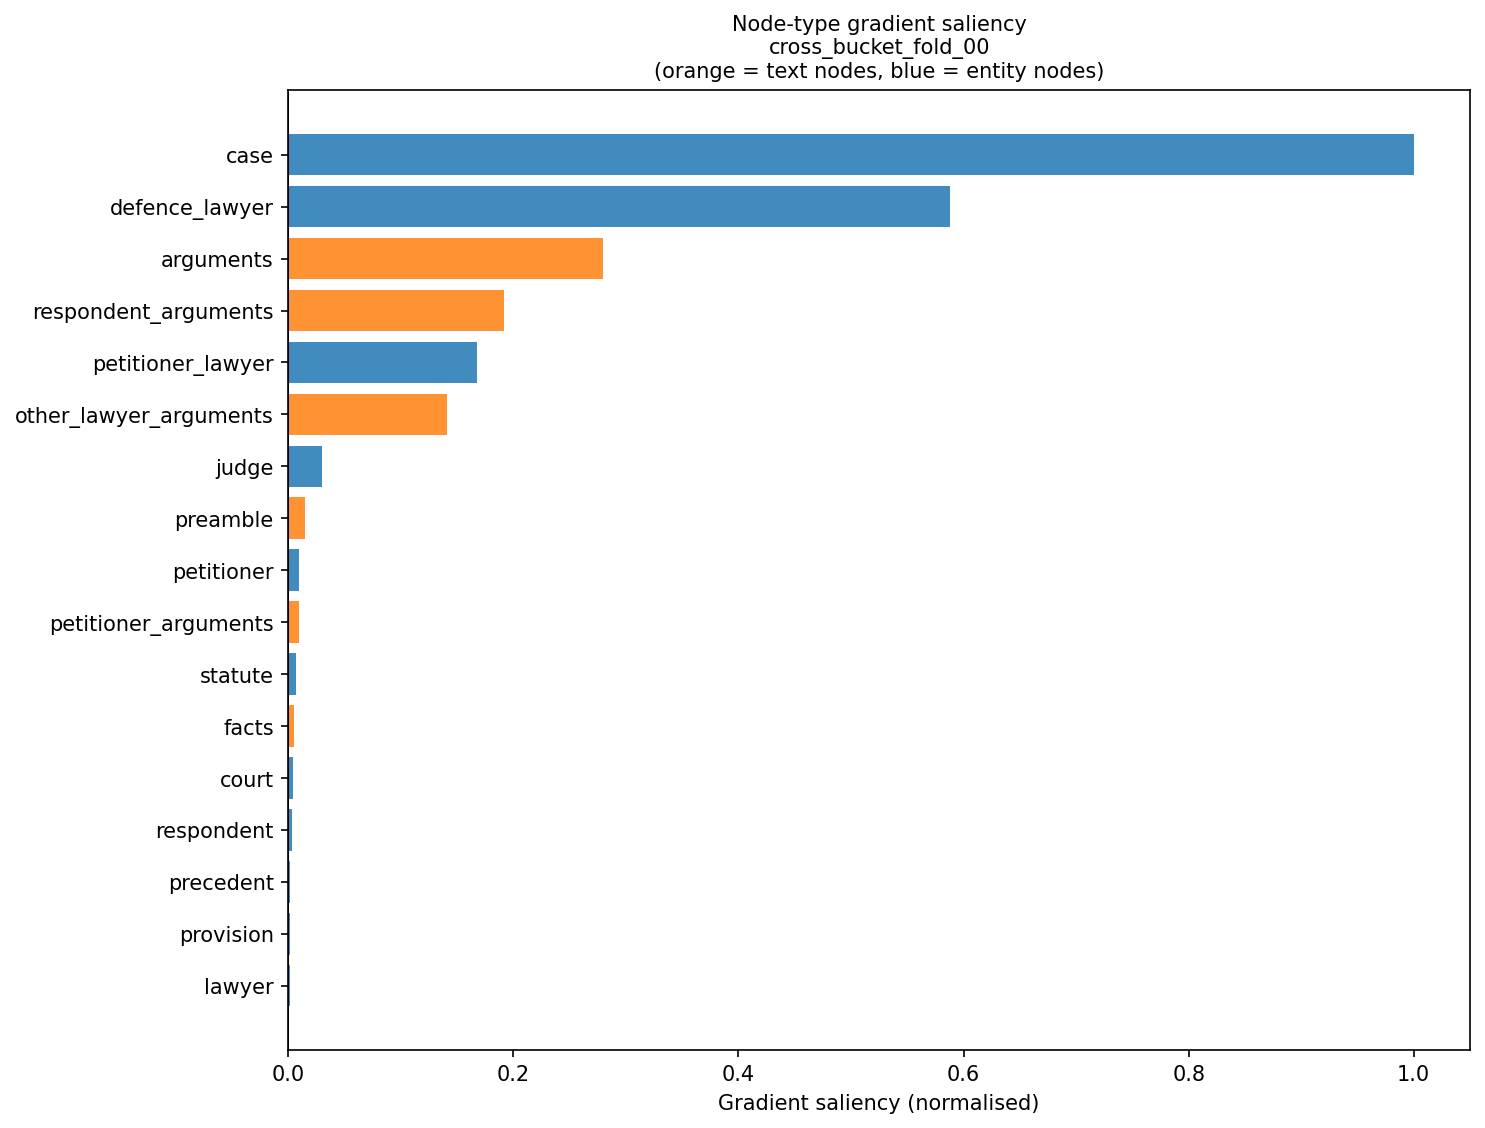
\includegraphics[width=\linewidth]{figures/explainability/gradient_saliency.png}
  \end{minipage}
  \caption{Edge-level attention (a) and node-type gradient saliency
  (b) on the cross-bucket baseline, fold~0. Reverse edges into the
  \textsc{Case} node dominate the attention mass; saliency
  concentrates on the argument-bearing text nodes.}
  \label{fig:attention_saliency}
\end{figure}

\section{Error Decomposition by Legal Domain and Year}
\label{app:error_domain_year}

Figure~\ref{fig:error_domain_year} decomposes test accuracy by legal
domain and by judgment year. Overall test accuracy is $0.8005$;
\emph{family~\&~matrimonial} is the strongest domain at $0.8254$,
\emph{motor~accidents} at $0.8209$; \emph{financial~fraud} at $0.7757$
and \emph{sexual~offences} at $0.7844$ are the weakest. This ordering
tracks structural properties of the buckets identified in
Chapter~\ref{chap:graph_exploration}: repetitive, highly-connected
sub-graphs are easier to generalise over than the doctrinally
heterogeneous fraud and sexual-offence cases, and largely restates
the per-bucket pattern already reported in
Chapter~\ref{chap:results}. After excluding the very earliest years
(small $n$, non-representative), per-year accuracy is flat: there is
no evidence of temporal drift in the model's behaviour.

\begin{figure}[H]
  \centering
  \begin{minipage}{0.49\textwidth}
    {\footnotesize (a) Accuracy by legal domain\par}
    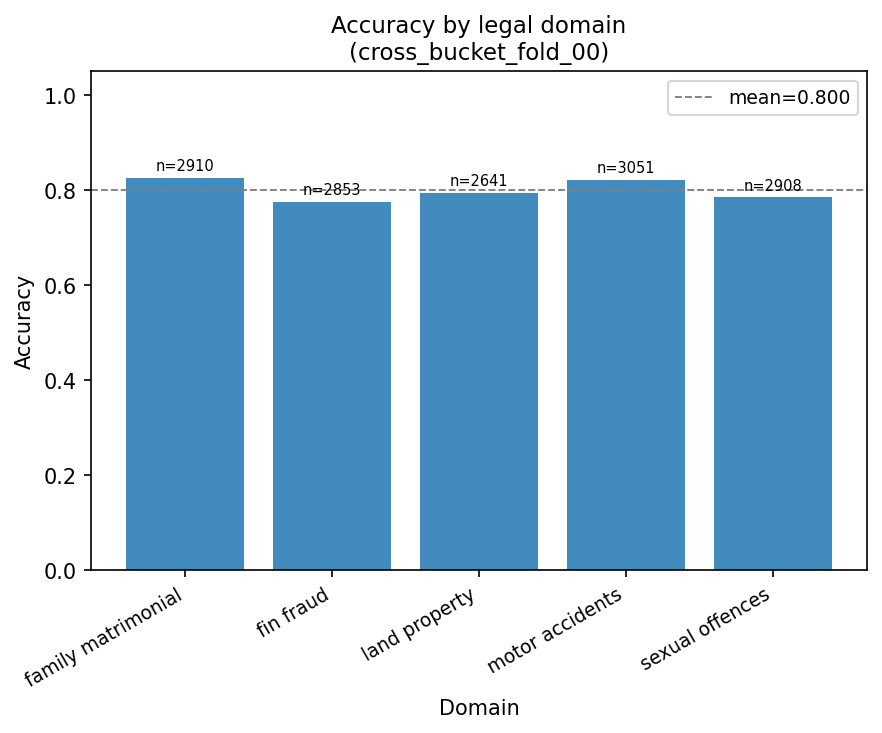
\includegraphics[width=\linewidth]{figures/explainability/error_by_domain.png}
  \end{minipage}\hfill
  \begin{minipage}{0.49\textwidth}
    {\footnotesize (b) Accuracy by judgment year\par}
    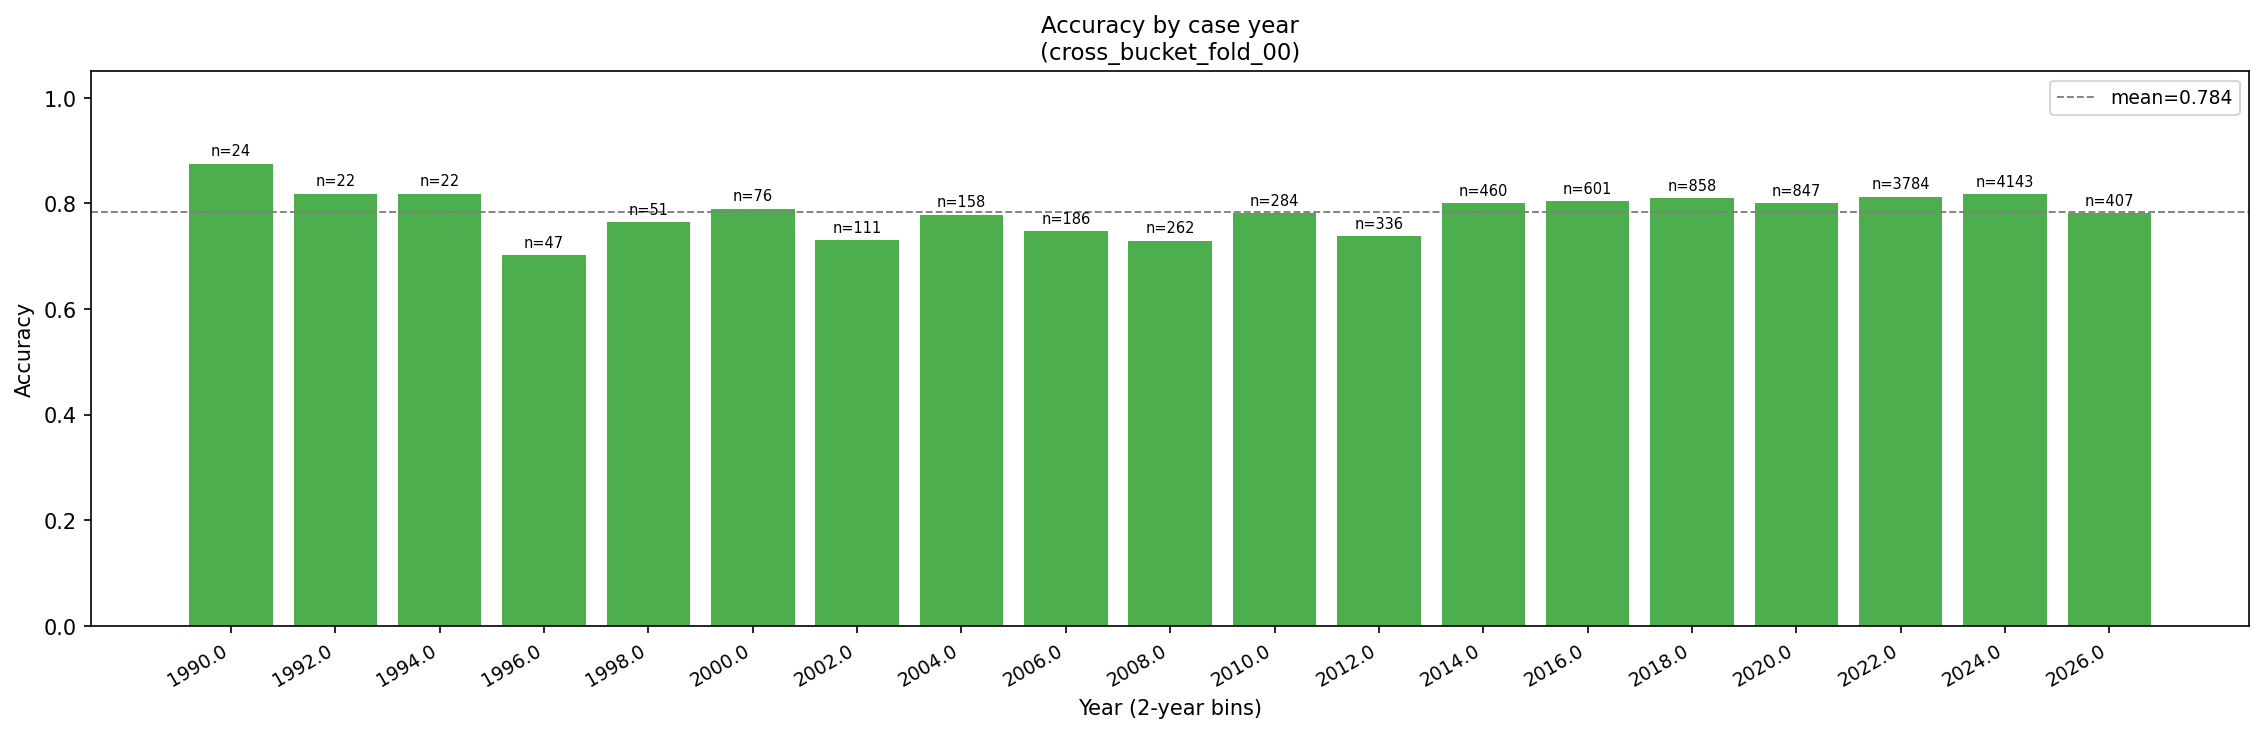
\includegraphics[width=\linewidth]{figures/explainability/error_by_year.png}
  \end{minipage}
  \caption{Error decomposition by legal domain and by year on the
  cross-bucket baseline (fold~0). Domain ordering is stable across
  ablations; year shows no systematic drift once the small-$n$ early
  years are excluded.}
  \label{fig:error_domain_year}
\end{figure}

\chapter{Supplementary Metrics: Accuracy and ROC-AUC}
\label{app:supplementary_metrics}

Macro-F1 is the primary metric throughout Chapter~\ref{chap:results}
because it is robust to the moderate outcome imbalance documented in
Section~\ref{sec:per_class_behaviour}. For completeness,
Table~\ref{tab:cross_bucket_accuracy} and
Table~\ref{tab:cross_bucket_rocauc} report accuracy and ROC-AUC of
the same variants on the same datasets. Because the task is
single-label binary, micro-F1 is numerically identical to accuracy
and is therefore omitted as a separate column.

\begin{table}[H]
  \centering
  \scriptsize
  \setlength{\tabcolsep}{3pt}
  \begin{adjustbox}{max width=\textwidth}
  \begin{tabular}{lccccccc}
    \toprule
    Model & Family & Fin.\ Fraud & Land/Prop. & Motor Acc. & Sexual Off. & Cross-bucket & Mean$_5$ \\
    \midrule
    \texttt{LR (no graph)}$^{\dagger}$ & 0.7762 & 0.7043 & 0.7280 & 0.7903 & 0.7171 & 0.7443 & 0.7432 \\
    \texttt{text\_only} & 0.8205\,$\pm$\,0.007 & 0.7635\,$\pm$\,0.008 & 0.8062\,$\pm$\,0.010 & 0.8249\,$\pm$\,0.004 & 0.7732\,$\pm$\,0.006 & 0.7732\,$\pm$\,0.006 & 0.7977 \\
    \texttt{baseline} (HGT) & 0.8217\,$\pm$\,0.008 & 0.7683\,$\pm$\,0.009 & 0.8083\,$\pm$\,0.005 & 0.8420\,$\pm$\,0.004 & 0.7752\,$\pm$\,0.007 & 0.7811\,$\pm$\,0.006 & 0.8031 \\
    \texttt{hierarchical\_enc} & \textbf{0.8275\,$\pm$\,0.009} & 0.7668\,$\pm$\,0.011 & 0.8029\,$\pm$\,0.010 & 0.8439\,$\pm$\,0.006 & \underline{0.7780\,$\pm$\,0.008} & 0.7811\,$\pm$\,0.003 & 0.8038 \\
    \texttt{section\_sep\_enc} & \underline{0.8270\,$\pm$\,0.009} & \textbf{0.7717\,$\pm$\,0.012} & 0.8104\,$\pm$\,0.009 & 0.8430\,$\pm$\,0.007 & 0.7745\,$\pm$\,0.008 & \underline{0.7892\,$\pm$\,0.009} & \textbf{0.8053} \\
    \textbf{\texttt{party\_args\_lr\_decay}} & 0.8254\,$\pm$\,0.003 & \underline{0.7709\,$\pm$\,0.011} & 0.8103\,$\pm$\,0.006 & 0.8413\,$\pm$\,0.003 & \textbf{0.7809\,$\pm$\,0.004} & \textbf{0.8020\,$\pm$\,0.004} & \underline{0.8058} \\
    \texttt{no\_names} & 0.8251\,$\pm$\,0.006 & 0.7702\,$\pm$\,0.011 & \underline{0.8104\,$\pm$\,0.011} & \textbf{0.8461\,$\pm$\,0.002} & 0.7743\,$\pm$\,0.010 & 0.7866\,$\pm$\,0.007 & 0.8052 \\
    \texttt{no\_cross\_case} & 0.8246\,$\pm$\,0.007 & 0.7688\,$\pm$\,0.013 & \textbf{0.8105\,$\pm$\,0.009} & 0.8418\,$\pm$\,0.003 & 0.7751\,$\pm$\,0.008 & 0.7837\,$\pm$\,0.005 & 0.8042 \\
    \texttt{case\_node\_minimised} & 0.8195\,$\pm$\,0.004 & 0.7678\,$\pm$\,0.009 & 0.8011\,$\pm$\,0.008 & \underline{0.8423\,$\pm$\,0.011} & 0.7750\,$\pm$\,0.006 & 0.7755\,$\pm$\,0.003 & 0.8011 \\
    \bottomrule
  \end{tabular}
  \end{adjustbox}
  \caption{Accuracy across all variants and domains, 5-fold mean
  $\pm$ sample standard deviation. \textbf{Bold} marks the best
  value per column; \underline{underline} marks the second-best.
  $^{\dagger}$\,\texttt{LR (no graph)} is reported on fold~0 from
  the probing pipeline.}
  \label{tab:cross_bucket_accuracy}
\end{table}

\begin{table}[H]
  \centering
  \scriptsize
  \setlength{\tabcolsep}{3pt}
  \begin{adjustbox}{max width=\textwidth}
  \begin{tabular}{lccccccc}
    \toprule
    Model & Family & Fin.\ Fraud & Land/Prop. & Motor Acc. & Sexual Off. & Cross-bucket & Mean$_5$ \\
    \midrule
    \texttt{text\_only} & 0.8944\,$\pm$\,0.005 & 0.8407\,$\pm$\,0.005 & 0.8638\,$\pm$\,0.004 & 0.8880\,$\pm$\,0.004 & \textbf{0.8495\,$\pm$\,0.004} & 0.8561\,$\pm$\,0.007 & 0.8673 \\
    \texttt{baseline} (HGT) & 0.8923\,$\pm$\,0.008 & 0.8406\,$\pm$\,0.006 & 0.8645\,$\pm$\,0.006 & 0.9010\,$\pm$\,0.005 & 0.8442\,$\pm$\,0.006 & 0.8674\,$\pm$\,0.002 & 0.8685 \\
    \texttt{hierarchical\_enc} & \underline{0.8963\,$\pm$\,0.009} & 0.8403\,$\pm$\,0.009 & \textbf{0.8676\,$\pm$\,0.007} & \underline{0.9037\,$\pm$\,0.007} & \underline{0.8462\,$\pm$\,0.007} & 0.8655\,$\pm$\,0.003 & \underline{0.8708} \\
    \texttt{section\_sep\_enc} & \textbf{0.8968\,$\pm$\,0.006} & \textbf{0.8416\,$\pm$\,0.011} & \underline{0.8676\,$\pm$\,0.005} & \textbf{0.9044\,$\pm$\,0.004} & 0.8441\,$\pm$\,0.006 & \underline{0.8712\,$\pm$\,0.008} & \textbf{0.8709} \\
    \textbf{\texttt{party\_args\_lr\_decay}} & 0.8940\,$\pm$\,0.006 & 0.8373\,$\pm$\,0.008 & 0.8625\,$\pm$\,0.007 & 0.9024\,$\pm$\,0.006 & 0.8436\,$\pm$\,0.006 & \textbf{0.8831\,$\pm$\,0.002} & 0.8680 \\
    \texttt{no\_names} & 0.8959\,$\pm$\,0.003 & \underline{0.8416\,$\pm$\,0.005} & 0.8640\,$\pm$\,0.009 & 0.9022\,$\pm$\,0.006 & 0.8441\,$\pm$\,0.007 & 0.8665\,$\pm$\,0.006 & 0.8695 \\
    \texttt{no\_cross\_case} & 0.8951\,$\pm$\,0.007 & 0.8410\,$\pm$\,0.008 & 0.8637\,$\pm$\,0.003 & 0.9031\,$\pm$\,0.002 & 0.8421\,$\pm$\,0.005 & 0.8658\,$\pm$\,0.002 & 0.8690 \\
    \texttt{case\_node\_minimised} & 0.8881\,$\pm$\,0.008 & 0.8332\,$\pm$\,0.008 & 0.8552\,$\pm$\,0.009 & 0.9020\,$\pm$\,0.005 & 0.8320\,$\pm$\,0.010 & 0.8560\,$\pm$\,0.001 & 0.8621 \\
    \bottomrule
  \end{tabular}
  \end{adjustbox}
  \caption{ROC-AUC across all variants and domains, 5-fold mean
  $\pm$ sample standard deviation. \textbf{Bold} marks the best
  value per column; \underline{underline} marks the second-best.}
  \label{tab:cross_bucket_rocauc}
\end{table}

The ranking divergence between Table~\ref{tab:cross_bucket_results}
and Table~\ref{tab:cross_bucket_rocauc} is informative. On per-domain
ROC-AUC, the encoder-side variants (\texttt{section\_sep\_enc},
\texttt{hierarchical\_enc}) produce the cleanest score distributions
and lead the per-bucket columns. On macro-F1 and on pooled accuracy,
\texttt{party\_args\_lr\_decay} dominates because its per-class
behaviour is more balanced once the threshold is fixed at $0.5$.
Both readings are consistent with the same underlying model: the
encoder variants produce the sharpest pre-threshold geometry, while
\texttt{party\_args\_lr\_decay} produces the best post-threshold
classification.
